% Rozdział 2. Wstęp teoretyczny
\chapter{Wstęp teoretyczny}
% Rozdział 2.1.  Modelowanie napędów elektrycznych
\section{Ujęcie systemowe napędu elektrycznego}
Rau Krishnan przedstawia napęd elektryczny w ujęciu systemowym, w postaci układu zmiennej prędkości złożonym z czterech elementów:
\begin{itemize}[label=$\bullet$, align=left, labelwidth=1.5em, leftmargin=!]
    \item Maszyny elektrycznej
    \item Przekształtnika mocy
    \item Sterownika - sterowanie silnikiem oraz przetwornicą mocy, tak aby spełniały wymagania obciążenia
    \item Obciążenie
\end{itemize}
Zdefiniowany w ten sposób napęd elektryczny zaprezentowany został za pomocą schematu blokowego, widocznego na rysunku nr. \ref{fig:Motor_Drive_PBD} \cite{krishnan2001electric}.
Jego komponenty składowe zostały w spośób skrócony opisane w dalszej częsci tego podrozdziału. \par
\vspace{1cm}
\begin{figure}[htbp]
    \centering
    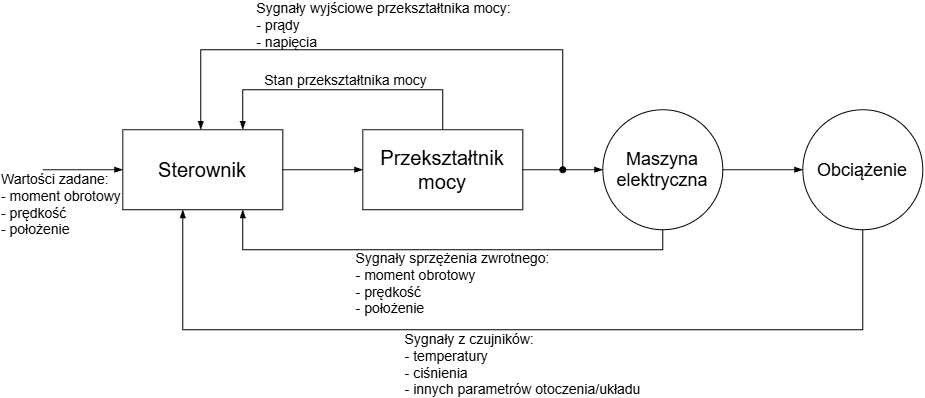
\includegraphics[width=16cm, height=6.6cm]{Obrazy/Electric_motor_drive_PBD.png
    }\par
    \caption{Schemat blokowy układu napędowego (opracowanie własne na podstawie \cite{krishnan2001electric}).}
    \label{fig:Motor_Drive_PBD}
\end{figure}
\vspace{1cm}
\subsection{Maszyna elektryczna}
W systemach zmiennej prędkości współcześnie stosuje się maszyny elektryczne, których zadaniem jest przekształcanie energii elektrycznej w mechaniczną.
Ze względu na zasadę działania oraz rodzaj zasilania podzielić je można na trzy rodzaje\cite{krishnan2001electric}:
\begin{itemize}[label=$\bullet$, align=left, labelwidth=1.5em, leftmargin=!]
    \item Maszyny prądu stałego (DC) - klasyfikowane na dwie główne grupy: komutatorowe (stosowane coraz rzadziej) oraz bezkomutatorowe (zwane również BLDC, współcześnie stosowane coraz częściej)\cite{grzesiak2016sterowanie}.
    \item Maszyny AC - mają największe znaczenie w aplikacjach przemysłowych, dzielone najczęściej na dwie grupy: asynchroniczne i synchroniczne\cite{grzesiak2016sterowanie}.
    \item Maszyny specjalne - maszyny reluktancyjne przełączalne.
\end{itemize}
\subsection{Przekształtnik mocy}
Maszyny elektryczne zasilane są przez przekształtniki mocy, które podzielić można na trzy grupy\cite{krishnan2001electric}:
\begin{itemize}[label=$\bullet$, align=left, labelwidth=1.5em, leftmargin=!]
    \item Prostowniki sterowane - przekształtniki, których zadaniem jest przekształcenie prądu przemiennego (AC) w prąd stały (DC).
    \item Falownik - przekształtniki, których zadaniem jest przekształcenie prądu stałego (DC) w prąd przemienny (AC).
    \item Cyklokonwertery - przekształtniki, których zadaniem jest przekształcenie prądu przemiennego (AC) na prąd przemienny (AC) o regulowanej wartości i regulowanej częstotliwości.
\end{itemize}
\subsection{Sterownik}
Napędy elektryczne wyposażone są również w sterowniki realizujące prawa sterowania, które uwzględniają charakterystyki obciążenia i silnika wraz z ich wzajemnymi oddziaływaniami.
Dopasowanie silnika i obciążenia odbywa się za pośrednictwem przekształtnika energoelektronicznego, w tym celu sterownik steruje jego wejściem\cite{krishnan2001electric}.\par
Sterowniki obsługują parametry wejść i wyjść, a więc wartości zadane oraz wielkości mierzone.
W zależności od zaprojektowanego układu, dane pomiarowe mogą obejmować wielkości takie jak położenie, prędkość, prąd czy moment obrotowy\cite{krishnan2001electric}\cite{lastowiecki2011napkedy}.
\subsection{Obciążenie}
Obciążenie maszyny elektrycznej (silnika) zdefiniować można jako wszystkie wartości wielkości mechanicznych odzwierciedlających wymagania, które stawiane są w danej chwili tej maszynie \cite{IEC60034-1_2022}.
Wymagania te, charakteryzują się zależnością momentu obciążenia od prędkości przedstawioną wzorem nr. \ref{eq:load} \cite{krishnan2001electric}.
\begin{equation}
    M_{\text{obc}} \propto \omega_m^x
    \label{eq:load}
\end{equation}

\section{Silnik komutatorowy D.C.}
